\newpage

\chapter{Мотивация и постановка задачи}\label{ch:chapter_1}

\section{Диаграммы связей}
Диаграмма связей реализуется в виде древовидной схемы, пример на
рис.~\ref{ris:mindmap}. \begin{figure}[h!] \centering
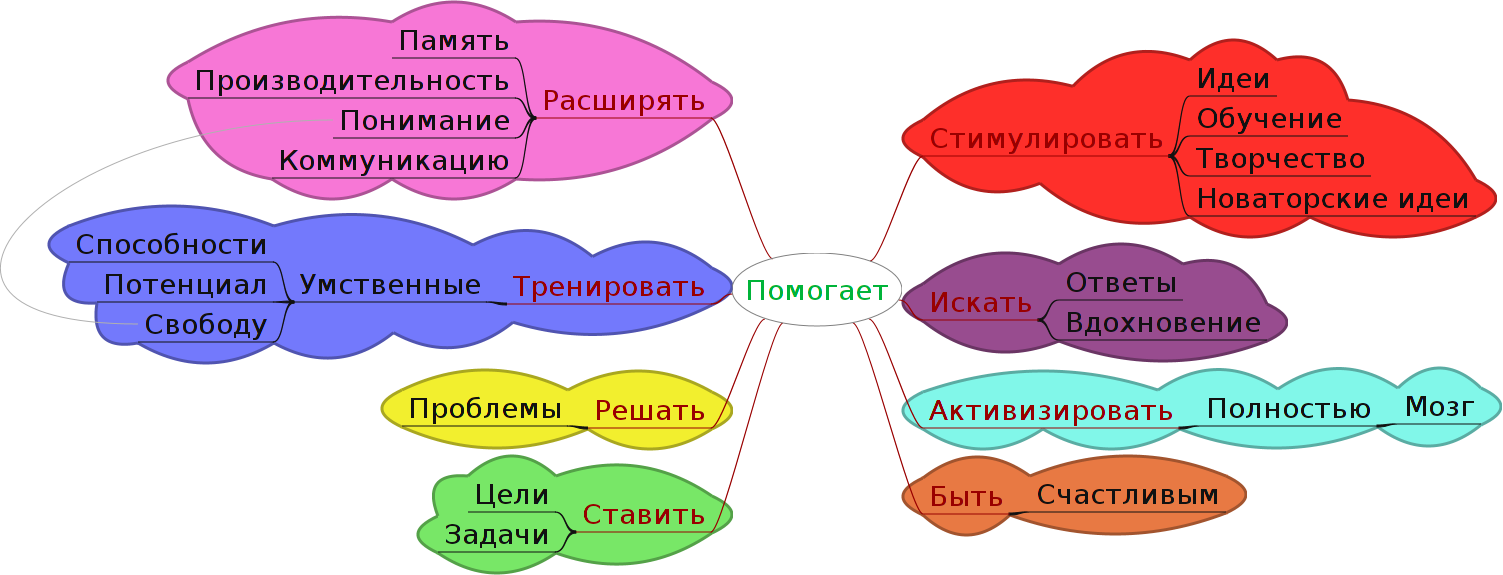
\includegraphics[width=1\linewidth]{mind-map}
\caption{Пример диаграммы связей}
\label{ris:mindmap}
\end{figure}

Возможность сворачивать узлы дает большее удобство для редактирования больших
диаграмм, возможность сосредоточиться на какой то отдельной части диаграммы. Так
же при различном оформлении отдельных узлов (цвет текста, цвет фона, рамка
вокруг текста, применение пиктограмм), соединительных линий можно повысить более
четкое разграничение различных частей диаграммы. Облака обычно применяются для
выделения очень важных ключевых идей. В диаграммах связей могут быть
использованы гиперссылки на веб-страницы, локальные файлы или адреса электронной
почты. Так же используются графические связи, чтобы показать взаимосвязь
элементов, находящихся в различных частях диаграммы. На рис. можно видеть пример
применения некоторых вышеописанных атрибутов узлов.

\section{Обзор существующих редакторов диаграмм связей}\label{sec:overview_of_mind_map}

В этом разделе производится обзор существующих редакторов диаграмм связей, а так
же оценка их применимости, достоинства и недостатки. Так как для некоторых
платформ существует больше редакторов, чем для других, то будут рассмотрены
самые популярные из них.

\subsection{Редакторы диаграмм для iPhone}

Мобильные устройства на платформе iPhone являются одними из самых
распространенных в мире, для данной платформы существует очень много приложений
для решения различных задач, в том числе существуют несколько приложений для
редактирования диаграмм связей.

Одно из известных приложений для редактирования диаграмм связей "--- это
MindNode. Данная программа имеет версии как для компьютера так и для iPhone, но
компьютерная версия программы реализована только для системы Mac OS X.

MindNode имеет однопользовательский интерфейс редактирования диаграммы, с
возможностью экспорта в различные форматы: формат MindNode, FreeMind, в виде
изображения формата .png, древовидный список в виде простого текста, а так же в
виде OPLM файла (язык разметки, основанный на XML).

Программа поддерживает работу как в вертикальном так и в горизонтальном режимах.
Диаграмму можно приближать и удалять. Так же программа поддерживает поиск текста
по узлам, реализована возможность изменять цвет связей,
создавать/переименовывать/удалять элементы, сортировать элементы схемы.

В целом программа удобна для использования. Однако, существенный минус ее "---
это цена. Программу можно приобрести в AppStore за \$5.99. Для того чтобы иметь
возможность синхронизации с компьютером, придется заплатить еще \$20.

Так же популярным редактором для платформы iPhone является редактор MindJet. У
данного приложения возможностей намного больше чем у MindNode. Отличительной
особенностью MindJet являются: работа с иконками, сворачивать и разворачивать
ветви, функции управления задачами "--- начальная и конечная даты выполнения
задачи. Цена на такую программу составляет около 6 евро.

\subsection{Редакторы диаграмм для платформы Android}

Платформа Android "--- одна из популярных платформ, основанная на ядре Linux.
Платформа базируется на Dalvik virtual machine, поэтому преимущества и
возможности операционной системы Linux на данной платформе практически не
используются.

MindMap memo "--- известный редактор диаграмм связей для платформы Android. Он
имеет скудную функциональность: масштабирование, копирование/вставка, изменение
цвета узла, работа с иконками, сворачивание/разворачивание веток, изменение
фона. Умеет экспортировать и импортировать файлы в формате FreeMind.

\subsection{Мультиплатформенные редакторы диаграмм}

MindMeister "--- одна из мощнейших Web 2.0 сервисов для мобильных устройств на
платформах iPhone и Maemo. Ее отличительные особенности это совместная работа
над диаграммой в режиме реального времени через интернет, так же возможна работа
в оффлайн режиме.

Программа взаимодействует с онлайновым сервисом Mindmeister который и реализует
хранение и совместную работу над диаграммами.

Из преимуществ стоит отметить очень широкий набор инструментов: иконки,
изменение цветов узлов, связей, фона, чат, поиск текста, SSL. Из недостатков
"--- бесплатная версия программы позволяет пользователю создавать до 3
интеллект-карт и импорт карт из FreeMind. Платные же версии стоят \$9 в месяц,
либо \$59 в год.

В данном классе приложений существует крайне мало бесплатных версий.
Функциональность некоторых из них очень бедны, в частности MindNode не умеет
работать с иконками, под платформу Maemo 5 вообще нет приложений такого типа,
более того, все рассмотренные приложения кроме MindMeister вообще не
поддерживают совместное редактирование диаграмм связей.

\section{Описание проекта}\label{sec:project_summary}

Совмещение таких технологий, как мобильные устройства и диаграммы связей "---
очень перспективно, в первую очередь для повышения мобильности участников,
которые работают над диаграммой. Так же это позволяет уменьшить затраты на
проведение совместной работы над диаграммами связей. Но в данный момент
инструментов под мобильные устройства практически нет. Поэтому было решено
создать проект по разработке приложения, которое обладало бы богатой
функциональностью и поддерживало режим совместного редактирования диаграмм.

Основной целью проекта является разработка редактора диаграмм связей с
поддержкой совместного редактирования диаграмм связей для мобильных устройств.
Редактор должен использовать формат FreeMind, для обеспечения свободного чтения
и редактирования файлов, созданных как на мобильных устройствах, так и на
настольных компьютерах.

Основные возможности:
\begin{itemize}
\item Чтение и запись файлов в формате FreeMind
\item Отображение диаграмм связей и навигация по ним
\begin{itemize}
\item Поддержка работы с несколькими диаграммами
\end{itemize}
\item Поддержка совместного редактирования диаграмм
\item Особенности пользовательского интерфейса
\begin{itemize}
\item Интернационализация
\item Использование клавиатуры и сенсорного дисплея
\end{itemize}
\end{itemize}

При совместной работе возникает необходимость коммуникации между членами группы. По этой причине в приложение должен быть встроен простейший сервис обмена текстовыми сообщениями.

Ввиду того, что проект предполагает полностью распределенную среду общения между устройствами, что является новым для данной категории приложений, то необходим поиск концепции эффективной модели совместного редактирования диаграмм связей.

\section{Обзор платформы Maemo 5}\label{sec:compare_platforms}

Для реализации проекта была выбрана платформа Maemo 5.
Maemo представляет собой встраиваемую ОС, разработанную на базе дистрибутивов Debian и предназначенную для устройств финской корпорации с процессорами ARM. Система основана на ядре GNU/Linux, свободно распространяемых программах, а также собственных разработках Nokia, многие из которых — закрыты. Другое важное отличие "--- Maemo не ориентирована, как Android, на Java-приложения и дает разработчикам большую свободу. В частности, на Maemo 4 были перенесены многие популярные открытые программы. Nokia выпускает и SDK для разработчиков приложений.

Архитектура системы. В нижней части программного стека располагается загрузчик NoLo (Nokia Loader), ядро GNU/Linux, которое управляет памятью, процессами, устройствами, файловой системой, осуществляет взаимодействие между процессами, а также предоставляет API программам, работающим в пространстве пользователя (т.н. userspace). В общем, все устроено как в любом другом дистрибутиве Linux, с учетом аппаратных особенностей устройств Nokia. Далее рассмотрим системные сервисы и основные библиотеки:
\begin{itemize}
\item
GLib — низкоуровневая библиотека, расширяющая возможности, стандартной библиотеки libc языка C (она служит основой для GTK+ и Gnome);
\item
D-Bus — шина сообщений, которая предоставляет приложениям широкий набор средств межпроцессного взаимодействия. Программа разрабатывается в рамках проекта freedesktop.org и активно используется во многих открытых проектах (например, в Gnome и KDE);
\item
HAL (Hardware Abstraction Layer) — демон, предоставляющий слой аппаратных абстракций. Первоначально был разработан в компании RedHat, сейчас HAL является частью все того же freedesktop.org;
X Window System — графическая подсистема, обеспечивающая возможность работы GUI-приложений.
\end{itemize}
 
На следующем уровне находятся библиотеки GTK+, а также необходимые для них средства (cairo, Pango и ATK).

На самом верхнем уровне находится среда рабочего стола Hildon, которая представляет из себя смесь компонентов Gnome, открытых разработок сообщества и собственных средств Nokia. Собственно, Hildon можно считать «мобильной» вариацией среды рабочего стола Gnome.

Недавно был анонсирован переход Maemo на графические библиотеки QT. При этом, GTK+/Hildon получит статус поддерживаемого сообществом. Понятно, что при таком серьезном изменении архитектуры следующий релиз системы не может быть развитием текущего. Тем не менее, MeeGo будет отличаться от Maemo 5 едва ли не сильнее, чем она сама — от Maemo 4. Т.е. разработка проекта уже разошлась на две независимых ветки и при всех несомненных достоинствах, Maemo 5 является не более чем переходной версией.

\section{Используемый инструментарий}\label{sec:choose_toolkit}

Nokia N900 "--- смартфон от компании Nokia, работающий под управлением операционной системы Maemo 5.
Nokia N900 является первым устройством, основанным на микропроцессоре TI OMAP3 с ядром ARM Cortex-A8.
В отличие от предыдущих интернет-планшетов компании, N900 является первым, обладающим функциями телефона.
Также аппарат работает как 5-мегапиксельная камера, портативный медиа-плеер и Интернет клиент с возможностью работы с электронной почтой и веб-браузером.
Он имеет 3.5-дюймовый резистивный сенсорный экран с разрешением 800х480 пикселей. Устройство снабжено тактильной (вибрация) и звуковой (клик) отдачей при вводе данных.
Смартфон имеет выдвижную трехстрочную подсвечиваемую клавиатуру.
В дополнение к английской QWERTY-раскладке, выдвижная клавиатура обеспечена итальянской, французской, немецкой, русской или финской/шведской раскладками.

Qt "--- кросс-платформенный инструментарий разработки ПО на языке программирования C++~\cite{qt_4, qt_4_with_examples}.
Существуют также «привязки» ко многим другим языкам программирования: Python (PyQt, PySide), Ruby (Qt-Ruby), Java (Qt Jambi), PHP (PHP-Qt) и другие.

Библиотека включает в себя все основные классы, которые могут потребоваться при разработке прикладного программного обеспечения, начиная от элементов графического интерфейса и заканчивая классами для работы с сетью, базами данных и XML. Qt является полностью объектно-ориентированным, легко расширяемым и поддерживающим технику компонентного программирования.

Python "--- высокоуровневый язык программирования общего назначения с акцентом на производительность разработчика и читаемость кода. Синтаксис ядра Python минималистичен. В тоже время стандартная библиотека включает большой объем полезных функций. Python поддерживает несколько парадигм программирования, в том числе структурное, объектно-ориентированное, функциональное, императивное и аспектно-ориентированное. Основные архитектурные черты --- это динамическая типизация, автоматическое управление памятью, полная интроспекция, механизм обработки исключений, поддержка многопоточных вычислений и удобные высокоуровневые структуры данных. Код в Python организовывается в функции и классы, которые могут объединяться в модули (которые в свою очередь могут быть объединены в пакеты)~\cite{python}.

PyQt "--- набор <<привязок>> графического фреймворка Qt для языка программирования Python, выполненный в виде расширения Python. PyQt практически полностью реализует возможности Qt. А это более 600 классов, более 6000 функций и методов. Модули входящие в набор: QtCore,
QtGui, QtNetwork, QtOpenGL, QtScript, QtSql, QtSvg, QtXml.

PySide "--- привязка языка Python к инструментарию Qt, совместимая на уровне API с PyQt. В отличие от PyQt PySide доступна для свободного использования как в открытых, так и закрытых, в частности, коммерческих, проектах, поскольку лицензирована по LGPL.

Проект возник в результате нежелания создателей PyQt менять лицензионную политику своего проекта.
Первая публичная версия PySide вышла в августе 2009 года. Основными разработчиками PySide являются программисты Nokia.

\section{Постановка задачи}\label{sec:statement_task}

Редактор диаграмм связей ориентирован на большую аудиторию пользователей, поэтому важной задачей представляется эргономика интерфейса пользователя и дизайн элементов управления.

В данный момент в проекте HiveMind имеются классы для работы с диаграммой связей, образующие ядро приложения, а так же классы для сохранения/загрузки диаграмм из файлов формата FreeMind.
В рамках данной работы решаются задачи разработки основных компонентов пользовательского интерфейса для модели диаграммы связей, а именно:
\begin{itemize}
\item
область графического представления диаграммы связей;
\item
контекстное меню, вызываемое на узлах диаграммы связей;
\item
диалог редактирования текста узла;
\item
диалог выбора пиктограмм.
\end{itemize}

При написании приложений под мобильные платформы требуется уделять особого внимания разработке пользовательского интерфейса. Вот основные отличия в построении интерфейса для мобильных устройств на платформе Maemo~5 от настольных компьютеров:
\begin{itemize}
\item малые размеры экрана (800х480 пикселей);
\item наличие сенсорного дисплея;
\item отсутствие манипулятора мышь;
\item особенности клавиатуры.
\end{itemize}

Ввиду специфики устройств разработан стандарт Hildon Guidlines~\cite{hildon}, направленный на унификацию пользовательского интерфейса для платформы Maemo~5. В частности при разработке пользовательского интерфейса должны выполняться следующие требования:
\begin{itemize}
\item Размеры кнопок должны быть не менее 64х64 пикселей;
\item Поддержка интернационализации;
\item Нельзя использовать иерархические структуры (деревья);
\item Нет инициализации фокуса в списках и меню.
\end{itemize}

Подводя итог, можно сказать, что разработка пользователького интерфейса для Maemo~5 очень специфична. Он должен быть стандартизирован, и в то же время требуется разработать эргономичный пользовательский интерфейс.